\documentclass[parskip=half]{scrartcl}
% ------------------------------------------------------------------------------
% LaTeX-Grundkonfiguration von Stefan Rothe
% ------------------------------------------------------------------------------

% 1 Konfiguration der Schriftarten
% --------------------------------
% um \ifXeTeX verwenden zu können
\usepackage{iftex}

\ifXeTeX
  % Setze PDF-Version auf 1.7
  \special{pdf:minorversion 7}

  % 1.1 Konfiguration der Schriftarten für XeTeX (empfohlen)
  % ----------------------------------------------------------
  \usepackage{fontspec}

  \IfFontExistsTF{Helvetica}{\setmainfont{Helvetica}}{%
    \IfFontExistsTF{Arial}{\setmainfont{Arial}}{}%
  }

  \IfFontExistsTF{Helvetica}{\setsansfont{Helvetica}}{%
    \IfFontExistsTF{Arial}{\setsansfont{Arial}}{}%
  }

  \IfFontExistsTF{Menlo}{\setmonofont[SizeFeatures={Size=10}]{Menlo}}{%
    \IfFontExistsTF{Courier New}{\setmonofont[SizeFeatures={Size=10}]{Courier New}}{}%
  }
\else
  % Setze PDF-Version auf 1.7
  \pdfminorversion=7

  % 1.2 Konfiguration der Schriftarten für PdfTeX
  % -----------------------------------------------

  % Unterstützung von UTF-8 (Unicode)
  \usepackage[utf8]{inputenc}

  % Unterstützung der modernen Zeichencodierung
  \usepackage[T1]{fontenc}

  % Moderne Schriftart verwenden
  \usepackage{lmodern}

  % Schriftart Helvetica verwenden
  \usepackage{helvet}

  % serifenfreie Schriftvariante verwenden
  \renewcommand{\familydefault}{\sfdefault}
\fi

% 2 wichtige Pakete laden und konfigurieren
% -----------------------------------------

% sprachspezifische Anpassungen
\usepackage[ngerman]{babel}

% Absatzabstände kontrollieren für nicht-KOMA-Klassen
\makeatletter
\@ifclassloaded{scrartcl}{}{\usepackage{parskip}}
\makeatother

% Aufzählungen
\usepackage{enumitem}

% mehrere Spalten
\usepackage{multicol}

% Rahmen
\usepackage{mdframed}

% Tabellen
\usepackage{booktabs}
\usepackage{tabularx}

% Grafiken (JPG, PNG, PDF)
\usepackage{graphicx}

% Links
\usepackage{hyperref}
\hypersetup{colorlinks=true,urlcolor=blue,linkcolor=black}

% Einbinden von Quellcode
\usepackage{listings}
\lstdefinestyle{mystyle}{
  basicstyle=\ttfamily,
  numberstyle=\scriptsize\color{black!70},
  numbers=left,
  numbersep=0.75cm
}
\lstset{style=mystyle}

% 3 Mathematik
% ------------

% 3.1 Zahlen und Einheiten schön darstellen
% -----------------------------------------
\usepackage{siunitx}
\sisetup{%
  mode=match,
  exponent-product=\cdot,
  group-digits=integer,
  group-separator={\text{\textquotesingle}}
}

% 3.2 AMS-Mathematik
% ------------------

\usepackage[fleqn]{amsmath}
\usepackage{amssymb}

% 3.3 Vektoren
% ------------
\usepackage[b]{esvect}

\makeatletter
% Koordinatenschreibweise für 2D-Punkte
\NewDocumentCommand\pxy@internal{mmm}{\mathopen{}\left(#1/#2\right)\mathclose{}}
\NewDocumentCommand\pxy{o>{\SplitArgument{2}{,}}m}{\IfNoValueF{#1}{#1}\pxy@internal #2}

% Komponentenschreibweise für 2D-Vektoren
\NewDocumentCommand\vxy@internal{mmm}{\begin{pmatrix}#1\\#2\end{pmatrix}}
\NewDocumentCommand\vxy{>{\SplitArgument{2}{,}}m}{\vxy@internal #1}
% Komponentenschreibweise für 3D-Vektoren
\NewDocumentCommand\vxyz{mmm}{\begin{pmatrix}#1\\#2\\#3\end{pmatrix}}
\makeatother

% Lineare Gleichungssysteme
\usepackage{systeme}
\sysdelim||

% Kürzen bei Brüchen zeigen
\usepackage{cancel}

% Schriftliche Division
\usepackage{longdivision}
\longdivisionkeys{style=german}

% eigene Operatoren
\DeclareMathOperator{\ggT}{ggT}
\DeclareMathOperator{\kgV}{kgV}
\DeclareMathOperator{\lb}{lb}

% muss wegen der Konfiguration vor tikz eingebunden werden
% Mit table können Tabellenzellen eingefärbt werden
\usepackage[table]{xcolor}
% für Geometrie (TikZ-Erweiterung)
% damit wird auch tikz eingebunden
\usepackage{tkz-base}
\usepackage{tkz-fct}
% Konfiguration Darstellung von Tangenten in tkz-fct
\tkzfctset{tan style/.style={red,thick,>=}}
\usepackage{tkz-euclide}
% Bäume mit tikz
\usepackage{forest}

% Material Design-Farben
% ----------------------
\definecolor{lightblue}{HTML}{BBDEFB} % MD Blue 100
\definecolor{lightred}{HTML}{FFCDD2} % MD Red 100
\definecolor{lightgrey}{HTML}{F5F5F5} % MD Gray 100
\definecolor{lightgreen}{HTML}{C8E6C9} % MD Green 100
\definecolor{lightorange}{HTML}{FFE0B2} % MD Orange 100

\definecolor{theoremcolor}{HTML}{FFEBEE} % MD Red 50
\definecolor{notecolor}{HTML}{FFECB3} % MD Amber 100

\definecolor{red}{HTML}{D50000} % MD Red A700
\definecolor{green}{HTML}{31843F} % MD Green A700
\definecolor{blue}{HTML}{2962FF} % MD Blue A700
\definecolor{teal}{HTML}{00BFA5} % MD Teal A700
\definecolor{cyan}{HTML}{00B8D4} % MD Cyan A700
\definecolor{yellow}{HTML}{EE8E0D} % WordPress Colors Yellow Fire 40%

\tikzset{dim style/.append style={purple,dashed}}
\tikzset{dim fence style/.append style={purple}}
\tikzset{mark angle style/.append style={german}}

% eigene Befehle
% --------------

\tikzset{circled/.style={shape=circle,draw,inner sep=2pt}}
\NewDocumentCommand\circled{m}{\tikz[baseline=(char.base)]{\node[circled] (char) {#1};}}

% Umgebung eqt
\NewDocumentEnvironment{eqt}{}{\begin{array}{>{\displaystyle}r@{\hspace{0.2cm}}>{\displaystyle}l@{\hspace{1cm}}|l}}{\end{array}}

% Makro \result, um das Resultat von Berechnungen hervorzuheben.
\NewDocumentCommand\result{m}{\textcolor{red}{#1}}

% Makro \extra, um schwierige Zusatzaufgaben zu markieren
\NewDocumentCommand\extra{}{$\bigstar\quad$}

\newmdenv[,skipabove=\parskip,outerlinewidth=1.5pt]{example}
\newmdenv[backgroundcolor=notecolor,skipabove=\parskip,outerlinewidth=1.5pt]{note}
\newmdenv[backgroundcolor=theoremcolor,skipabove=\parskip,outerlinewidth=1.5pt]{theorem}
\newmdenv[backgroundcolor=theoremcolor,outerlinewidth=1.5pt]{instructions}

\usepackage{fontawesome5}
\def\digital{\faLaptop{} }
\def\present{\faTrophy{} }

\def\rosconfig{1}


\usepackage{scrlayer-scrpage}
\pagestyle{scrheadings}




\KOMAoption{DIV}{12}
\KOMAoption{toc}{listof}
\DeclareTOCStyleEntry[entryformat=\bfseries,beforeskip=2pt,linefill=\TOCLineLeaderFill]{tocline}{section}
\setcounter{tocdepth}{1}

\title{Vektorgeometrie 1}
\author{Stefan Rothe}
\date{07.09.2024}

\newpairofpagestyles{firstpage}{%
  \cofoot{\textcopyright{} Gymnasium Kirchenfeld\\Dieses Skript steht unter einer Creative Commons Attribution 4.0 International-Lizenz.\\(CC BY 4.0)}
}

\makeatletter
\lohead{\@title}
\rohead{\@date}
\cofoot{\thepage}
\rofoot{}
\makeatother

\begin{document}
  \maketitle
  \thispagestyle{firstpage}
  \begin{center}
    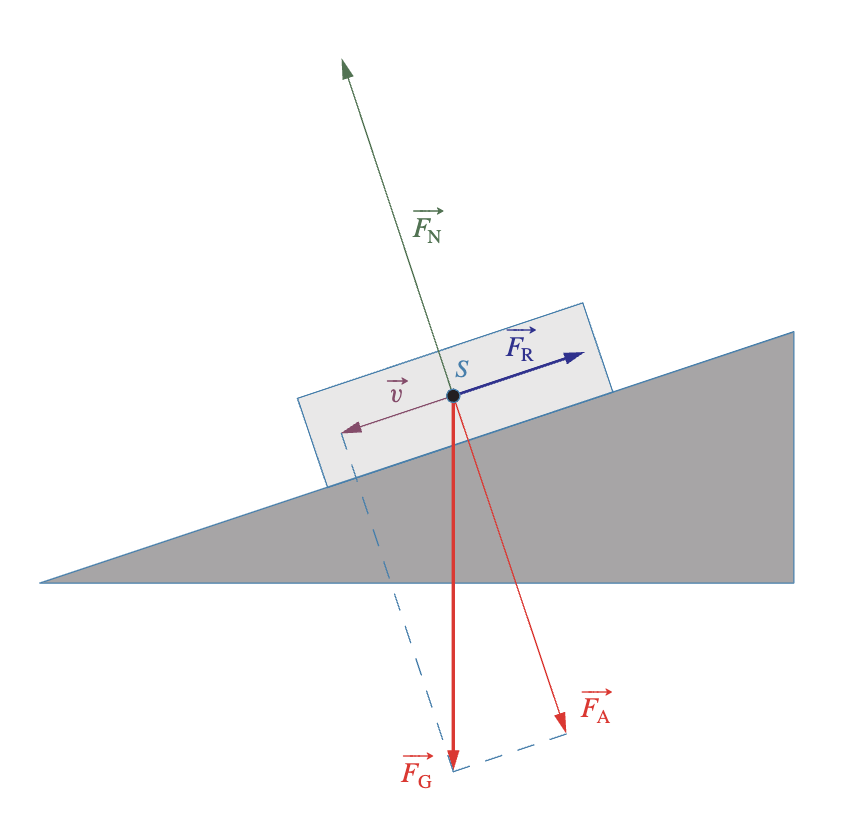
\includegraphics[width=0.6\textwidth]{title.png}
  \end{center}
  \tableofcontents
  \newpage
  \input{Einführung}
  \newpage
\section{Komponentendarstellung}

% ------------------------------------------------------------------------------
\subsection{Komponenten}

Wird ein Vektor $\vv{v}$ in das kartesische Koordinatensystem eingezeichnet, so kann der Vektor beschrieben werden durch die
\[
  \vv{v} = \vxy{v_{x}}{v_{y}}
\]
Dabei werden $v_{x}$ und $v_{y}$ die Komponenten des Vektors $\vv{v}$ genannt. $v_{x}$ ist die horizontale Komponente, $v_{y}$ die vertikale Komponente. Die horizontale Komponente steht oben, die vertikale Komponente unten.

% ------------------------------------------------------------------------------
\subsection{Addition und Subtraktion}
Die Addition und Subtraktion von Vektoren erfolgt komponentenweise.

\begin{theorem}
  \textbf{Addition.} Zwei Vektoren $\vv{a} = \vxy{a_{x}}{a_{y}}$ und $\vv{b} = \vxy{b_{x}}{b_{y}}$ werden addiert, indem ihre Komponenten addiert werden:
  \[
    \vv{a}+\vv{b} = \vxy{a_{x}}{a_{y}}+\vxy{b_{x}}{b_{y}} = \vxy{a_{a}+b_{x}}{a_{y}+b_{y}}
  \]
  \textbf{Subtraktion.} $\vv{a}$ und $\vv{b}$ werden subtrahiert, indem ihre Komponenten subtrahiert werden:
  \[
    \vv{a}-\vv{b} = \vxy{a_{x}}{a_{y}}-\vxy{b_{x}}{b_{y}} = \vxy{a_{a}-b_{x}}{a_{y}-b_{y}}
  \]

\end{theorem}

% ------------------------------------------------------------------------------
\subsection{Skalierung}

Die Skalierung eines Vektors erfolgt komponentenweise.

\begin{theorem}
  \textbf{Skalierung.} Ein Vektor  $\vv{a} = \vxy{a_{x}}{a_{y}}$ wird skaliert, indem seine Komponenten mit dem Faktor multipliziert werden:
  \[
    k\cdot\vv{a} = k\cdot\vxy{a_{x}}{a_{y}} = \vxy{k\cdot a_{a}}{k\cdot a_{y}}
  \]
\end{theorem}

% ------------------------------------------------------------------------------
\subsection{Länge}

Die Länge eines Vektors $\vv{a}$ wird mit $|\vv{a}|$ bezeichnet. Die Komponenten bilden zusammen mit dem Vektor ein rechtwinkliges Dreieck. Deshalb kann die Länge mit Hilfe des Satzes von Pythagoras aus dem Komponenten berechnet werden.

\begin{center}
  \begin{tikzpicture}
    \tkzInit[xmin=-4,xmax=8,ymin=-1,ymax=4]
    \tkzGrid[color=lightgray]
    \tkzDefPoint(0,0){S}
    \tkzDefPoint(5,3){Z}
    \tkzDefPoint(5,0){H}
    \tkzDrawSegment[thick,vector style](S,Z)
    \tkzDrawPolySeg[thick,red](S,H,Z)
    \tkzLabelSegment[above left](S,Z){$\vv{a}$}
    \tkzLabelSegment[red,below](S,H){$a_{x}$}
    \tkzLabelSegment[red,right](H,Z){$a_{y}$}
    \tkzMarkRightAngle[red,german,size=0.5](Z,H,S)
  \end{tikzpicture}
\end{center}

\begin{theorem}
  \textbf{Länge eines Vektors.} Die Länge $|\vv{a}|$ eines Vektors $\vv{a} = \vxy{a_{x}}{a_{y}}$ wird wie folgt berechnet:
  \[
    |\vv{a}| = \sqrt{a_{x}^{2}+a_{y}^{2}}
  \]
\end{theorem}

\begin{example}
  \textbf{Beispiel:} In der oben stehenden Abbildung hat der Vektor $\vv{a}$ die Komponenten $\vxy{5}{3}$. Also ist seine Länge
  \[
    |\vv{a}| = \sqrt{5^{2}+3^{2}} = \sqrt{34} \approx 5.831
  \]
\end{example}

% ------------------------------------------------------------------------------
\subsection{Nullvektor}

Ein spezieller Vektor ist der Nullvektor. Er stellt einen Pfeil der Länge Null dar. Im Gegensatz zu allen anderen Vektoren hat der Nullvektor keine Richtung. Der Nullvektor wird als Zahl Null mit einem Vektorpfeil geschrieben: $\vv{0}$. Alle seine Komponenten sind Null.
\[
  \vv{0} = \vxy{0}{0}
\]

% ------------------------------------------------------------------------------
\subsection{Gleichheit}

Zwei Vektoren sind genau dann gleich, wenn ihre Komponenten übereinstimmen:
\[
  \vxy{a_{x}}{a_{y}} = \vxy{b_{x}}{b_{y}} \qquad\Leftrightarrow\qquad a_{x} = b_{x} \quad\text{und}\quad a_{y} = b_{y}
\]
  \newpage
\section{Vektoren und Punkte}

\subsection{Unterschiede}
Vektoren und Punkte sind unterschiedliche Objekte mit unterschiedlichen Eigenschaften.

Ein \textbf{Punkt} befindet sich an einem bestimmten Ort und er hat keine Richtung. Ein Punkt $P$ mit den \textbf{Koordinaten} $x$ und $y$ wird wie folgt geschrieben:
\[
  \pxy[P]{x,y}
\]

Ein \textbf{Vektor} kann beliebig verschoben werden, er hat also keine feste Position, aber er zeigt in eine bestimmte Richtung. Ein Vektor $\vv{v}$ mit den \textbf{Komponenten} $v_{x}$ und $v_{y}$ wird folgendermassen geschrieben:
\[
  \vv{v} = \vxy{v_{x},v_{y}}
\]

% ------------------------------------------------------------------------------
\subsection{Ortsvektor}

Wird ein Vektor $\vv{OP}$ mit dem Ursprung $O$ als Anfangspunkt und dem Punkt $\pxy[P]{x,y}$ als Endpunkt definiert wird, so entsprechen die Komponenten des Vektors gerade den Koordinaten des Punkts $P$:
\[
  \vv{OP} = \vxy{x-0,y-0} = \vxy{x,y}
\]
\begin{center}
  \begin{tikzpicture}
    \tkzInit[xmin=0,xmax=8,ymin=0,ymax=4]
    \tkzAxeXY[]
    \tkzGrid[color=lightgray]
    \tkzDefPoint(0,0){O}
    \tkzDefPoint(6,2){P}

    \tkzDrawSegment[red,thick,vector style](O,P)
    \tkzLabelSegment[red,above left](O,P){$\vv{OP}=\vxy{x,y}$}

    \tkzDrawPoints(O,P)
    \tkzLabelPoint[above right](O){$O$}
    \tkzLabelPoint[above right](P){$P\pxy{x,y}$}
  \end{tikzpicture}
\end{center}

Dieser Vektor wird \textbf{Ortsvektor} des Punkts $P$ genannt. Der Ortsvektor von $P$ zeigt vom Ursprung $O$ zum Punkt $P$.

Werden Vektoren als Verschiebungen aufgefasst, so verschiebt der Ortsvektor den Ursprung $O$ in den Punkt $P$.
\begin{example}
  \textbf{Beispiel:} Der Ortsvektor des Punkts $\pxy[A]{-3,5}$ lautet $\vv{OA} = \vxy{-3,5}$.
\end{example}

% ------------------------------------------------------------------------------
\subsection{Vektor zwischen Punkten}

Ein Vektor kann durch einen Anfangspunkt $A$ und einen Endpunkt $B$ bestimmt werden.

\begin{center}
  \begin{tikzpicture}
    \tkzInit[xmin=0,xmax=12,ymin=0,ymax=4]
    \tkzAxeXY[]
    \tkzGrid[color=lightgray]
    \tkzDefPoint(0,0){O}
    \tkzDefPoint(2,3){A}
    \tkzDefPoint(9,1){B}

    \tkzDrawSegment[vector style](O,A)
    \tkzLabelSegment[above left](O,A){$\vv{OA}$}

    \tkzDrawSegment[vector style](O,B)
    \tkzLabelSegment[above left](O,B){$\vv{OB}$}

    \tkzDrawSegment[red,thick,vector style](A,B)
    \tkzLabelSegment[red,above right](A,B){$\vv{AB}$}

    \tkzDrawPoints(A,B)
    \tkzLabelPoint[left](A){$A\pxy{x_{A},y_{A}}$}
    \tkzLabelPoint[right](B){$B\pxy{x_{B},y_{B}}$}
  \end{tikzpicture}
\end{center}
Der Vektor $\vv{AB}$, welcher von Punkt $A$ nach Punkt $B$ zeigt, kann als Subtraktion der Ortsvektoren von $A$ und $B$ ausgedrückt werden.
\[
  \vv{AB} = \vv{OB} - \vv{OA} = \vxy{x_{B},y_{B}} - \vxy{x_{A},y_{A}} = \vxy{x_{B}-x_{A},y_{B}-y_{A}}
\]
Daraus lässt sich schliessen, dass sich die Komponenten des Vektors $\vv{AB}$ durch Subtraktion der Koordinaten von Punkt $B$ und Punkt $A$ ergeben.


\begin{theorem}
  \textbf{Vektor aus Punkten.} Hat ein Vektor $\vv{AB}$ den Anfangspunkt $\pxy[A]{x_{A},y_{A}}$ und den Endpunkt $\pxy[B]{x_{B},y_{B}}$ besitzt, so lautet seine Komponentendarstellung
  \[
    \vv{AB} = \vxy{x_{B}-x_{A},y_{B}-y_{A}}
  \]
\end{theorem}

\begin{example}
  \textbf{Beispiel:} Im der oben stehenden Abbildung ist der Vektor $\vv{v}$ durch den Anfangspunkt $\pxy[A]{2,3}$ und den Endpunkt $\pxy[B]{9,1}$ definiert. Also lautet seine Komponentendarstellung
  \[
    \vv{AB} = \vxy{9-2,1-3} = \vxy{7,-2}
  \]
\end{example}

  \newpage
\section{Kollinearität und Orthogonalität}

Eine wichtige Frage ist es, ob zwei Vektoren parallel zueinander sind oder senkrecht aufeinander stehen.

\subsection{Kollinearität (parallel)}

Sind zwei Vektoren parallel, so werden sie als kollinear bezeichnet. Zwei Vektoren $\vv{a}$ und $\vv{b}$ sind parallel, wenn Sie in die gleiche oder umgekehrte Richtung zeigen. Das ist genau dann der Fall, wenn der eine Vektor ein vielfaches des anderen Vektors ist.

\begin{theorem}
  \textbf{Kollinearität.} Zwei Vektoren $\vv{a} = \vxy{a_{x}}{a_{y}}$ und $\vv{b} = \vxy{b_{x}}{b_{y}}$ sind kollinear (parallel), wenn es eine Zahl $\lambda$ gibt, sodass
  \[
    \vv{a} = \lambda\cdot\vv{b} \qquad\Leftrightarrow\qquad \vxy{a_{x}}{a_{y}} = \lambda\cdot\vxy{b_{x}}{b_{y}}
  \]
\end{theorem}

\begin{center}
  \begin{tikzpicture}
    \tkzInit[xmin=0,xmax=12,ymin=0,ymax=4]
    \tkzAxeXY[]
    \tkzGrid[color=lightgray]

    \tkzDefPoint(1,3){A1}
    \tkzDefShiftPoint[A1](2,-1){A2}
    \tkzDrawSegment[red,thick,-LaTeX](A1,A2)
    \tkzLabelSegment[red,above right](A1,A2){$\vv{a}$}

    \tkzDefPoint(9,1){B1}
    \tkzDefShiftPoint[B1](-6,3){B2}
    \tkzDrawSegment[red,thick,-LaTeX](B1,B2)
    \tkzLabelSegment[red,above right](B1,B2){$\vv{b}$}

    \tkzDefPoint(3,0){C1}
    \tkzDefShiftPoint[C1](2,2){C2}
    \tkzDrawSegment[thick,-LaTeX](C1,C2)
    \tkzLabelSegment[below right](C1,C2){$\vv{c}$}
  \end{tikzpicture}
\end{center}

\begin{example}
  \textbf{Beispiele:} Die Vektoren $\vv{a} = \vxy{2}{-1}$ und $\vv{b} = \vxy{-6}{3}$ sind kollinear, da:
  \[
     2 = \mathcolor{red}{-\frac{1}{3}\cdot} (-6) \qquad\qquad -1 = \mathcolor{red}{-\frac{1}{3}\cdot} 3
  \]

  Die Vektoren $\vv{a} = \vxy{2}{-1}$ und $\vv{c} = \vxy{2}{2}$ sind nicht parallel, da
  \[
    2 = \mathcolor{red}{1\cdot} 2 \qquad\qquad -1 = \mathcolor{red}{-\frac{1}{2}\cdot} 2
  \]
\end{example}

% ------------------------------------------------------------------------------
\subsection{Orthogonalität (senkrecht)}

Stehen zwei Vektoren senkrecht zueinander, so werden sie als \textbf{orthogonal} bezeichnet.

\begin{theorem}
  \textbf{Orthogonalität.} Zwei Vektoren $\vv{a} = \vxy{a_{x}}{a_{y}}$ und $\vv{b} = \vxy{b_{x}}{b_{y}}$ sind orthogonal (stehen senkrecht zueinander), wenn
  \[
    a_{x}\cdot b_{x}+a_{y}\cdot b_{y} = 0
  \]
\end{theorem}

\begin{center}
  \begin{tikzpicture}
    \tkzInit[xmin=0,xmax=12,ymin=0,ymax=4]
    \tkzAxeXY[]
    \tkzGrid[color=lightgray]

    \tkzDefPoint(1,3){A1}
    \tkzDefShiftPoint[A1](2,-3){A2}
    \tkzDrawSegment[red,thick,-LaTeX](A1,A2)
    \tkzLabelSegment[red,below left](A1,A2){$\vv{a}$}

    \tkzDefPoint(3,0){B1}
    \tkzDefShiftPoint[B1](6,4){B2}
    \tkzDrawSegment[red,thick,-LaTeX](B1,B2)
    \tkzLabelSegment[red,below right](B1,B2){$\vv{b}$}

    \tkzDefPoint(3,0){C1}
    \tkzDefShiftPoint[C1](1,4){C2}
    \tkzDrawSegment[thick,-LaTeX](C1,C2)
    \tkzLabelSegment[below right](C1,C2){$\vv{c}$}

    \tkzMarkRightAngle[red,german,size=0.5](B2,B1,A1)
  \end{tikzpicture}
\end{center}

\begin{example}
  \textbf{Beispiele:} Die Vektoren $\vv{a} = \vxy{2}{-3}$ und $\vv{b} = \vxy{6}{4}$ sind orthogonal, da:
  \[
    2\cdot 6 + (-3)\cdot 4 = 12 - 12 = 0
  \]
  Die Vektoren $\vv{a} = \vxy{2}{-3}$ und $\vv{c} = \vxy{1}{4}$ sind nicht orthogonal, da
  \[
    2\cdot 1 + (-3)\cdot 4 = 2-12 = -10 \ne 0
  \]
\end{example}

Ist ein Vektor in Komponentenform gegeben, so können die zu ihm senkrechten Vektoren einfach ermittelt werden:

\begin{theorem}
  \textbf{Senkrechter Vektor.} Ist der Vektor $\vv{a} = \vxy{a_{x}}{a_{y}}$ gegeben, so stehen die Vektoren
  \[
    \vxy{-a_{y}}{a_{x}} \qquad\qquad \vxy{a_{y}}{-a_{x}}
  \]
  senkrecht auf $\vv{a}$ und haben die gleiche Länge wie $\vv{a}$. Die Komponenten der senkrechten Vektoren erhält man, indem die Komponenten von $\vv{a}$ vertauscht werden und eine Komponente negiert wird.
\end{theorem}
Das lässt sich einfach überprüfen:
\begin{align*}
  a_{x}\cdot(-a_{y})+a_{y}\cdot a_{x} = -a_{x}\cdot a_{y}+a_{y}\cdot a_{x} &= 0 \\
  a_{x}\cdot a_{y}+a_{y}\cdot(-a_{x}) = a_{x}\cdot a_{y}-a_{y}\cdot a_{x} &= 0
\end{align*}

\begin{center}
  \begin{tikzpicture}
    \tkzInit[xmin=0,xmax=10,ymin=0,ymax=5]
    \tkzAxeXY[]
    \tkzGrid[color=lightgray]

    \tkzDefPoint(5,3){A1}
    \tkzDefShiftPoint[A1](2,-3){A2}
    \tkzDrawSegment[thick,-LaTeX](A1,A2)
    \tkzLabelSegment[below left](A1,A2){$\vv{a}$}

    \tkzDefShiftPoint[A1](3,2){B2}
    \tkzDrawSegment[red,thick,-LaTeX](A1,B2)
    \tkzLabelSegment[red,above left](A1,B2){$\vv{b}$}

    \tkzDefShiftPoint[A1](-3,-2){C2}
    \tkzDrawSegment[red,thick,-LaTeX](A1,C2)
    \tkzLabelSegment[red,above left](A1,C2){$-\vv{b}$}

    \tkzMarkRightAngle[red,german,size=0.5](C2,A1,A2)
  \end{tikzpicture}
\end{center}

\begin{example}
  \textbf{Beispiel:} Zum $\vv{a} = \vxy{2}{-3}$ stehen die folgenden beiden Vektoren senkrecht:
  \[
    \vv{b} = \vxy{3}{2} \qquad\qquad -\vv{b} = \vxy{-3}{-2}
  \]
\end{example}

  \newpage
\section{Anwendungen}

Mit Vektoren können geometrische Probleme algebraisch gelöst werden. Hier werden
exemplarisch ein paar solcher Probleme betrachtet.

% ------------------------------------------------------------------------------
\subsection{Streckenteilung}
\textbf{Aufgabe:} Teilen Sie die Strecke $\overline{AB}$ in drei gleiche Teile.
\[
  \pxy[A]{2,4} \qquad \pxy[B]{11,1}
\]
Zunächst wird der Vektor $\vv{a} = \vv{AB}$ bestimmt. Der erste Teilpunkt
$T_{1}$ erhält man, indem ein Drittel von $\vv{a}$ zum Ortsvektor von $A$
addiert wird. Der zweite Teilpunkt erhält man durch Addieren von zwei Dritteln
von $\vv{a}$.
\[
  \vv{a} := \vv{AB} \qquad\qquad \vv{OT_{1}} = \vv{OA} + \frac{1}{3}\vv{a} \qquad\qquad \vv{OT_{2}} = \vv{OA} + \frac{2}{3}\vv{a}
\]
\begin{center}
  \begin{tikzpicture}
    \tkzInit[xmin=0,xmax=12,ymin=0,ymax=5]
    \tkzAxeXY[]
    \tkzGrid[color=lightgray]
    \tkzDefPoint(0,0){O}
    \tkzDefPoint(2,4){A}
    \tkzDefPoint(11,1){B}
    \tkzDefPoint(5,3){T1}
    \tkzDefPoint(8,2){T2}
    \tkzDrawSegment[](A,B)
    \tkzDrawSegment[vector style](O,A)
    \tkzDrawSegment[vector style](O,T1)
    \tkzDrawSegment[vector style](O,T2)
    \tkzDrawSegment[red,thick,vector style](A,T1)
    \tkzDrawSegment[red,thick,vector style](T1,T2)
    \tkzDrawSegment[red,thick,vector style](T2,B)

    \tkzLabelSegment[above left](O,A){$\vv{OA}$}
    \tkzLabelSegment[above left](O,T1){$\vv{OT_{1}}$}
    \tkzLabelSegment[below right](O,T2){$\vv{OT_{2}}$}
    \tkzLabelSegment[red,below left](A,T1){$\frac{1}{3}\vv{a}$}
    \tkzLabelSegment[red,below left](T1,T2){$\frac{1}{3}\vv{a}$}
    \tkzLabelSegment[red,below left](T2,B){$\frac{1}{3}\vv{a}$}

    \tkzDrawPoints(A,B)
    \tkzDrawPoints[red](T1,T2)
    \tkzLabelPoint[above right](A){$A$}
    \tkzLabelPoint[above right](B){$B$}
    \tkzLabelPoint[red,above right](T1){$T_{1}$}
    \tkzLabelPoint[red,above right](T2){$T_{2}$}
  \end{tikzpicture}
\end{center}
Damit ergeben sich folgende Ortsvektoren und Koordinaten für $T_{1}$ und $T_{2}$:
\begin{align*}
       \vv{a} &= \vv{AB} = \vxy{11,1} - \vxy{2,4} = \vxy{11-2,1-4} = \vxy{9,-3} \\[2mm]
  \vv{OT_{1}} &= \vxy{2,4}+\frac{1}{3}\vxy{9,-3} = \vxy{2+\frac{1}{3}9,4+\frac{1}{3}(-3)} = \vxy{5,3} \\[2mm]
  \vv{OT_{2}} &= \vxy{2,4}+\frac{2}{3}\vxy{9,-3} = \vxy{2+\frac{2}{3}9,4+\frac{2}{3}(-3)} = \vxy{8,2}
\end{align*}
Die Strecke wird also durch die Punkte $\pxy[T_{1}]{5,3}$ und $\pxy[T_{2}]{8,2}$ in drei gleiche Teile geteilt.

% ------------------------------------------------------------------------------
\subsection{Umfang eines Dreiecks}
\textbf{Aufgabe:} Bestimmen Sie den Umfang des Dreiecks $\triangle ABC$ mit
\[
  \pxy[A]{3,2} \qquad \pxy[B]{8,1} \qquad \pxy[C]{7,4}
\]
Zwischen den Punkten $A$, $B$ und $C$ können die Vektoren $\vv{AB}$, $\vv{BC}$ und $\vv{CA}$ definiert werden.
\begin{center}
  \begin{tikzpicture}
    \tkzInit[xmin=0,xmax=12,ymin=0,ymax=5]
    \tkzAxeXY[]
    \tkzGrid[color=lightgray]
    \tkzDefPoint(3,2){A}
    \tkzDefPoint(8,1){B}
    \tkzDefPoint(7,4){C}
    \tkzDrawSegment[red,thick,vector style](A,B)
    \tkzDrawSegment[red,thick,vector style](B,C)
    \tkzDrawSegment[red,thick,vector style](C,A)
    \tkzLabelSegment[red,below left](A,B){$\vv{a}$}
    \tkzLabelSegment[red,above right](B,C){$\vv{b}$}
    \tkzLabelSegment[red,above left](C,A){$\vv{c}$}

    \tkzDrawPoints(A,B,C)
    \tkzLabelPoint[below left](A){$A$}
    \tkzLabelPoint[below right](B){$B$}
    \tkzLabelPoint[above](C){$C$}
  \end{tikzpicture}
\end{center}
Anschliessend werden die Längen der Vektoren ermittelt und addiert, um den Umfang des Dreiecks zu erhalten.
\begin{align*}
  \vv{a} &= \vv{AB} = \vxy{8-3,1-2} = \vxy{5,-1} & |\vv{a}| &= \sqrt{5^{2}+(-1)^{2}} = \sqrt{26} \approx 5.099 \\[2mm]
  \vv{b} &= \vv{BC} = \vxy{7-8,4-1} = \vxy{-1,3} & |\vv{b}| &= \sqrt{(-1)^{2}+3^{2}} = \sqrt{10} \approx 3.162 \\[2mm]
  \vv{c} &= \vv{CA} = \vxy{3-7,2-4} = \vxy{-4,-2} & |\vv{c}| &= \sqrt{(-4)^{2}+(-2)^{2}} = \sqrt{20} \approx 4.472
\end{align*}
Damit ergibt sich für den Umfang des Dreiecks:
\[
  U = |\vv{a}|+|\vv{b}|+|\vv{c}| \approx 5.099 + 3.162 + 4.472 \approx 12.733
\]

\newpage
% ------------------------------------------------------------------------------
\subsection{Schwerpunkt eines Dreiecks}
\textbf{Aufgabe:} Bestimmen den Schwerpunkt der Dreiecks $\triangle ABC$ mit
\[
  \pxy[A]{2,2} \qquad \pxy[B]{9,1} \qquad \pxy[C]{6,5}
\]
\begin{center}
  \begin{tikzpicture}
    \tkzInit[xmin=0,xmax=12,ymin=0,ymax=5]
    \tkzAxeXY[]
    \tkzGrid[color=lightgray]
    \tkzDefPoint(2,2){A}
    \tkzDefPoint(9,1){B}
    \tkzDefPoint(7,4){C}
    \tkzDefMidPoint(B,C) \tkzGetPoint{M}
    \tkzDefTriangleCenter[centroid](A,B,C)
    \tkzGetPoint{S}

    \tkzDrawSegment[thick](A,B)
    \tkzDrawSegment[thick](C,A)
    \tkzDrawSegment[vector style](O,A)
    \tkzDrawSegment[vector style](O,B)
    \tkzDrawSegment[red,thick,vector style](B,C)
    \tkzDrawSegment[red,thick,vector style](A,M)

    \tkzLabelSegment[above left](O,A){$\vv{OA}$}
    \tkzLabelSegment[below right,pos=0.6](O,B){$\vv{OB}$}
    \tkzLabelSegment[red,above left](A,M){$\vv{AM}$}
    \tkzLabelSegment[red,above right,pos=0.3](B,C){$\vv{b}$}

    \tkzDrawPoints(A,B,C,M,S)
    \tkzLabelPoint[above left](A){$A$}
    \tkzLabelPoint[below right](B){$B$}
    \tkzLabelPoint[above](C){$C$}
    \tkzLabelPoint[above right](M){$M$}
    \tkzLabelPoint[above right](S){$S$}
  \end{tikzpicture}
\end{center}
Zunächst wird der Vektor $\vv{b}$ ermittelt, welcher die Seite $b$ beschreibt.
\[
  \vv{b} = \vv{BC} = \vxy{7-9,4-1} = \vxy{-2,3} \\
\]
Nun kann der Mittelpunkt der Seite $b$ berechnet werden:
\[
  \vv{OM} = \vv{OB}+\tfrac{1}{2}\vv{b} = \vxy{9,1}+\tfrac{1}{2}\vxy{-2,3} = \vxy{8,2.5}
\]
Jetzt wird der Vektor $\vv{AM}$ berechnet, welcher die Seitenhalbierende beschreibt.
\[
  \vv{AM} = \vv{OM}-\vv{OA} = \vxy{8,2.5}-\vxy{2,2} = \vxy{6,0.5}
\]
Da der Schwerpunkt die Seitenhalbierende im Verhältnis 2:1 teilt, kann nun dessen Ortsverktor berechnet werden.
\[
  \vv{OS} = \vv{OA}+\tfrac{2}{3}\vv{AM} = \vxy{2,2}+\tfrac{2}{3}\vxy{6,0.5} = \vxy{6,2.\overline{3}}
\]
Der Schwerpunkt des Dreiecks hat also die Koordinaten $\pxy[S]{6,2.\overline{3}}$.
\newpage
% ------------------------------------------------------------------------------
\subsection{Parallelogramm}

\textbf{Aufgabe:} Ermitteln Sie den fehlenden Eckpunkt $C$ und den Umfang des Parallelogramms $ABCD$ mit
\[
  \pxy[A]{3,2} \qquad \pxy[B]{8,1} \qquad \pxy[D]{6,4}
\]
Zuerst werden die Seitenvektoren des Parallelogramms bestimmt:
\begin{align*}
  \vv{a} &= \vv{OB}-\vv{OA} = \vxy{8,1}-\vxy{3,2} = \vxy{8-3,1-2} = \vxy{5,-1} \\[2mm]
  \vv{b} &= \vv{OD}-\vv{OA} = \vxy{6,4}-\vxy{3,2} = \vxy{6-3,4-2} = \vxy{3,2}
\end{align*}
Der Punkt $C$ erhält man, indem der Punkt $B$ um den Vektor $\vv{b}$ verschiebt. Dazu wird $\vv{b}$ zum Ortsvektor $\vv{OB}$ addiert:
\[
  \vv{OC} = \vv{OB} + \vv{b} = \vxy{8,1} + \vxy{3,2} = \vxy{8+3,1+2} = \vxy{11,3}
\]
Also ist der vierte Punkt des Parallelogramms $\pxy[C]{11,3}$.

\begin{center}
  \begin{tikzpicture}
    \tkzInit[xmin=0,xmax=12,ymin=0,ymax=5]
    \tkzAxeXY[]
    \tkzGrid[color=lightgray]
    \tkzDefPoint(0,0){O}
    \tkzDefPoint(3,2){A}
    \tkzDefPoint(8,1){B}
    \tkzDefPoint(11,3){C}
    \tkzDefPoint(6,4){D}

    \tkzDrawSegment[vector style](O,A)
    \tkzLabelSegment[above left](O,A){$\vv{OA}$}

    \tkzDrawSegment[vector style](O,B)
    \tkzLabelSegment[below right](O,B){$\vv{OB}$}

    \tkzDrawSegment[thick,vector style](A,B)
    \tkzLabelSegment[below left](A,B){$\vv{a}$}

    \tkzDrawSegment[thick,vector style](A,D)
    \tkzLabelSegment[above left](A,D){$\vv{b}$}

    \tkzDrawSegment[red,thick,vector style](B,C)
    \tkzLabelSegment[red,below right](B,C){$\vv{b}$}

    \tkzDrawSegment[red,thick,dotted](C,D)

    \tkzDrawPoints(A,B,D)
    \tkzDrawPoints[red](C)
    \tkzLabelPoint[above left](A){$A$}
    \tkzLabelPoint[below right](B){$B$}
    \tkzLabelPoint[red,right](C){$C$}
    \tkzLabelPoint[above](D){$D$}
  \end{tikzpicture}
\end{center}

Der Umfang des Parallelogramms ergibt sich, indem die Längen von $\vv{a}$ und $\vv{b}$ addiert und verdoppelt werden:
\[
  U = 2\left(|\vv{a}| + |\vv{b}|\right) = 2\left(\sqrt{5^{2}+(-1)^2}+\sqrt{3^{2}+2^{2}}\right) \approx 2\cdot 8.704 \approx 12.310
\]

\newpage
% ------------------------------------------------------------------------------
\subsection{Quadrat}

\textbf{Aufgabe:} Ermitteln Sie die fehlenden Eckpunkte $C$ und $D$ sowie die Fläche des Quadrats $ABCD$ mit
\[
  \pxy[A]{3,2} \qquad \pxy[B]{6,1}
\]
\begin{center}
  \begin{tikzpicture}
    \tkzInit[xmin=0,xmax=10,ymin=0,ymax=5]
    \tkzAxeXY[]
    \tkzGrid[color=lightgray]
    \tkzDefPoint(3,2){A}
    \tkzDefPoint(6,1){B}
    \tkzDefPoint(7,4){C}
    \tkzDefPoint(4,5){D}
    \tkzDrawSegment[thick,vector style](A,B)
    \tkzLabelSegment[below left](A,B){$\vv{a}$}

    \tkzDrawSegment[red,thick,vector style](A,D)
    \tkzLabelSegment[red,above left](A,D){$\vv{b}$}
    \tkzDrawSegment[red,thick,vector style](B,C)
    \tkzLabelSegment[red,below right](B,C){$\vv{b}$}
    \tkzDrawSegment[red,thick,dotted](C,D)

    \tkzDrawPoints(A,B,D)
    \tkzDrawPoints[red](C)
    \tkzLabelPoint[left](A){$A$}
    \tkzLabelPoint[below](B){$B$}
    \tkzLabelPoint[red,right](C){$C$}
    \tkzLabelPoint[red,above](D){$D$}
    \tkzMarkRightAngle[red,german,size=0.5](B,A,D)
  \end{tikzpicture}
\end{center}
Zunächst wird der Vektor $\vv{a} = \vv{AB}$ ermittelt:
\[
  \vv{a} = \vxy{6,1}-\vxy{3,2} = \vxy{6-3,1-2} = \vxy{3,-1}
\]
Nun wird der zu $\vv{a}$ senkrechte Vektor $\vv{b}$ ermittelt:
\[
  \vv{b} = \vxy{1,3}
\]
Nun werden $C$ und $D$ ermittelt:
\begin{align*}
  \vv{OC} &= \vv{OB}+\vv{b} = \vxy{6,1} + \vxy{1,3} = \vxy{6+1,1+3} = \vxy{7,4} \\[2mm]
  \vv{OD} &= \vv{OA}+\vv{b} = \vxy{3,2} + \vxy{1,3} = \vxy{3+1,2+3} = \vxy{4,5}
\end{align*}
Die gesuchten Punkte sind also $\pxy[C]{7,4}$ und $\pxy[D]{4,5}$. Die Fläche des Quadrats beträgt
\[
  A = |\vv{a}|^{2} = \left(\sqrt{3^{2}+1^{2}}\right)^{2} = 9+1 = 10
\]

\newpage
% ------------------------------------------------------------------------------
\subsection{Kreis}

\textbf{Aufgabe:} Berechnen Sie den Mittelpunkt und den Radius des Kreises, auf welchem die folgenden drei Punkte liegen:
\[
  \pxy[A]{3,2} \qquad \pxy[B]{6,5} \qquad \pxy[C]{7,2}
\]
\begin{center}
  \begin{tikzpicture}
    \tkzInit[xmin=0,xmax=10,ymin=0,ymax=6]
    \tkzAxeXY[]
    \tkzGrid[color=lightgray]
    \tkzDefPoint(3,2){A}
    \tkzDefPoint(6,5){B}
    \tkzDefPoint(7,2){C}
    \tkzDefPoint(5,3){M}

    \tkzDrawCircle[thick,red](M,C)

    \tkzDrawSegment[red,thick,vector style](A,M)
    \tkzLabelSegment[red,below right](A,M){$\vv{AM}$}

    \tkzDrawPoints(A,B,C)
    \tkzDrawPoints[red](M)
    \tkzLabelPoints[below left](A)
    \tkzLabelPoints[above right](B)
    \tkzLabelPoints[below right](C)
    \tkzLabelPoints[red,below right](M)
  \end{tikzpicture}
\end{center}
Sei $\vv{OA}$ der Ortsvektor des Punkts $A$ auf dem Kreis und $\vv{OM}$ der Ortsvektor des Mittelpunkts $M$ mit den folgenden Komponenten:
\[
  \vv{OA} = \vxy{3,2} \qquad \vv{OM} = \vxy{x,y}
\]
Der Vektor $\vv{AM} = \vv{OM}-\vv{OA}$ zeigt vom Punkt $P$ zum Kreismittelpunkt $M$. Seine Länge ist der Radius des Kreises $r$:
\[
  \left|\vv{OM}-\vv{OA}\right| = r
\]
In Komponentenschreibweise ergibt sich die folgende Gleichung:
\[
  \sqrt{\left(x-3\right)^{2}+\left(y-2\right)^{2}} = r
\]
Um die Wurzel zu eliminieren wird die Gleichung quadriert.
\[
  \left(x-3\right)^{2}+\left(y-2\right)^{2} = r^{2}
\]
Für die Punkte $B$ und $C$ ergeben sich zwei analoge Gleichungen. Diese ergeben zusammen ein Gleichungssystem mit drei Gleichungen und drei Unbekannten:
\begin{align*}
  (x-3)^{2}+(y-2)^{2} &= r^{2} && \circled{1} \\
  (x-6)^{2}+(y-5)^{2} &= r^{2} && \circled{2} \\
  (x-7)^{2}+(y-2)^{2} &= r^{2} && \circled{3}
  \intertext{Die Gleichungen werden ausmultipliziert:}
  x^{2}-6x+y^{2}-4y+13 &= r^{2} && \circled{1} \\
  x^{2}-12x+y^{2}-10y+61 &= r^{2} && \circled{2} \\
  x^{2}-14x+y^{2}-4y+53 &= r^{2} && \circled{3} \\
\end{align*}
Durch Gleichsetzen der Gleichungen werden $r$ und die Quadrate eliminiert und es entsteht ein lineares Gleichungssystem:
\begin{align*}
  -6x-4y+13 &= -12x-10y+61 && \circled{1}=\circled{2} \\
  -6x-4y+13 &= -14x-4y+53 && \circled{1}=\circled{3}
  \intertext{Nach Zusammenfassen ergibt sich:}
  6x+6y &= 48 \\
  8x &= 40
\end{align*}
Die Lösung des Gleichungssystems ist $x = 5$ und $y = 3$. Also hat der Mittelpunkt des Kreises die Koordinaten $\pxy[M]{5,3}$.

Den Radius des Kreises ist die Länge des Vektors $\vv{AM}$:
\[
  r = \left|\vv{AM}\right| = \left|\vxy{5-2,3-2}\right| = \left|\vxy{3,1}\right| = \sqrt{3^{2}+1^{2}} = \sqrt{10} \approx 3.162
\]

\end{document}
